\chapter{Algorithms}
\label{ch:algorithms}



\section{Intuition}
\label{sec:intuition}

To solve this problem we have to evaluate all possible edge combinations. Even for greedy heuristics we need to limit the edge candidates. The algorithm considers high-degree vertices of each polarized community. This is motivated by the tendency that social graphs resemble a star-graphs. That means a small number of nodes with high popularity are connected with a lot of low popularity nodes. Garimella Et Al \cite{garimella} uses this star like topology to count the decrease of the polarization. While the intuition behind this process is the same we use a different metric. Garimella Et Al uses a random-walk controversy score while we use the polarization index$\pi(z)$.
\\
\\
Let $G$ be our social network graph. In the figure~\ref{fig:starA} bellow we can see how it resemble a star like shaped network. Nodes $0-4$ have an internal value of $Z_i = 1$ and nodes $5-9$ have an internal value of $Z_i=-1$. Now we are going to compute the polarization index for the network $G$. 
\\

\begin{figure}[t]
	\centering
	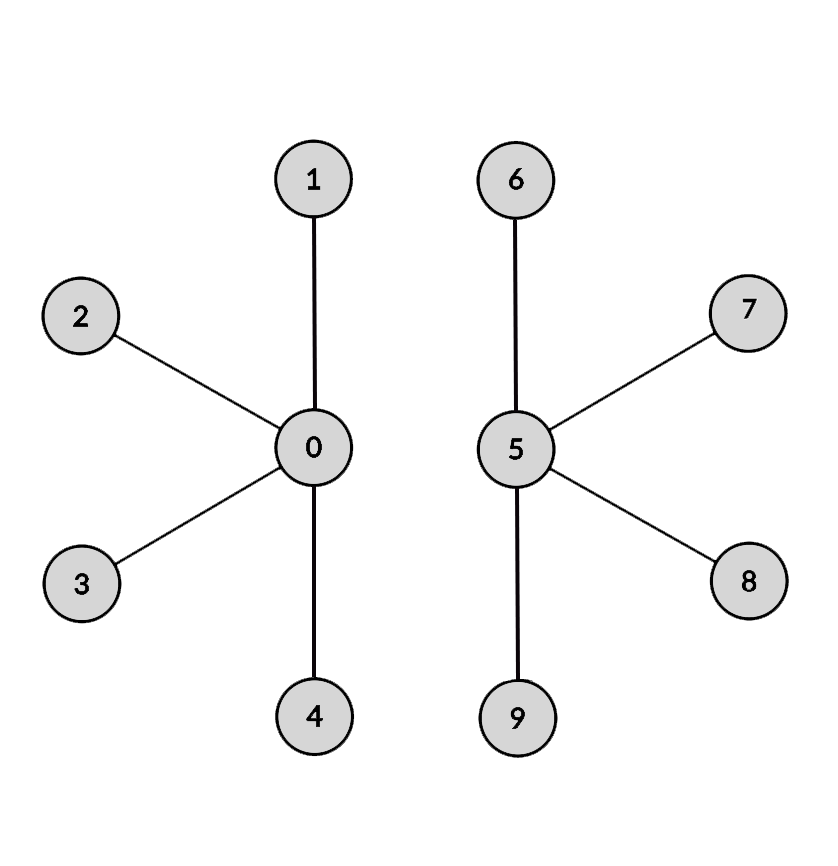
\includegraphics[width=0.65\textwidth]{Figures/starA}
	\caption{A star like graph with two communities.}
	\label{fig:starA}
\end{figure}

\begin{equation}
Z_0 = \frac{1*(1) + 4*(1)}{1 + 4} = \frac{5}{5} = 1
\end{equation}

\begin{equation}
Z_1,Z_2,Z_3,Z_4 = \frac{1*(1) + 1*(1)}{1 + 1} = \frac{2}{2} = 1
\end{equation}

\begin{equation}
Z_5 = \frac{1*(-1) + 4*(-1)}{1 + 4} = \frac{-5}{5} = -1
\end{equation}

\begin{equation}
Z_6,Z_7,Z_8,Z_9 = \frac{1*(-1) + 1*(-1)}{1 + 1} = \frac{-2}{2} = -1
\end{equation}

\begin{equation}
||\pi(z)||^2 = \frac{\sqrt{10}}{10} = 0.316227766
\end{equation}
\\

There are four edge additions that we consider. Connecting the center nodes or the most popular nodes of each polarized community together by connecting node $0$ with node $5$ $(case 1)$. Connecting the center node of the one side of the polarized community with a non central node by connecting node $0$ with node $6$ $(case 2)$and in a respectively for the other polarized community node $5$ with node $4$ $(case 3)$. Finally connecting non central nodes together by connecting node $1$ with node $9$ $(case 4)$.
We will now compute the reduction of each case.


\begin{figure}[t]
	\centering
	\begin{subfigure}[t]{0.3\textwidth}
		\centering
		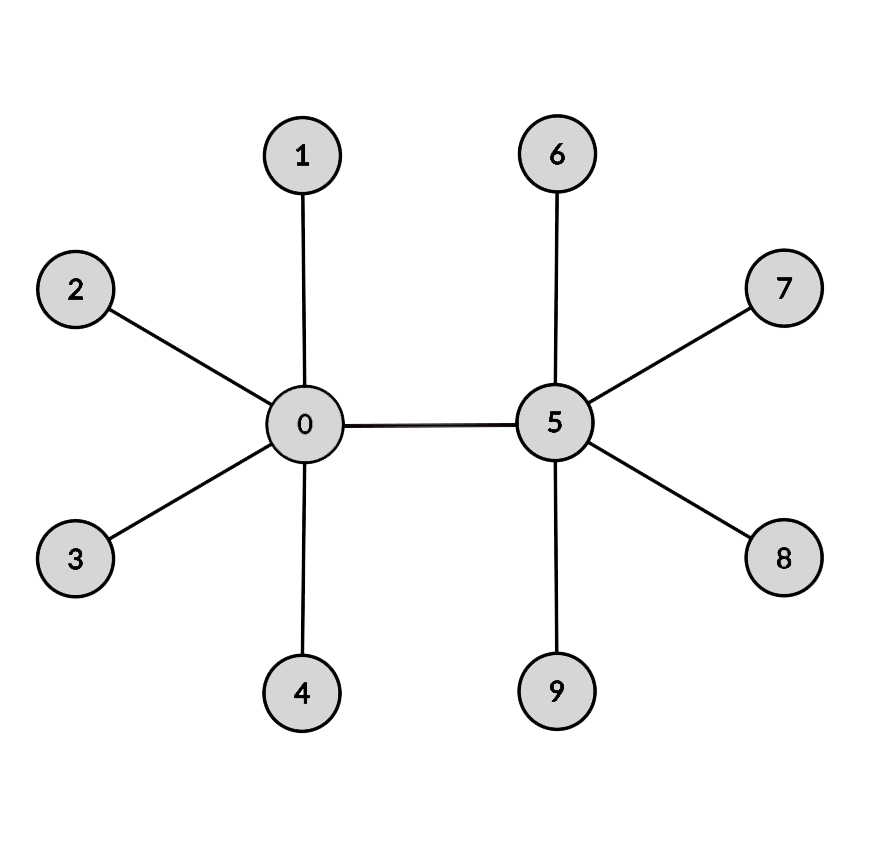
\includegraphics[height=0.15\textheight]{Figures/starB}
		\caption{}
		\label{subfig:starB}
	\end{subfigure}
	\hfill
	\begin{subfigure}[t]{0.3\textwidth}
		\centering
		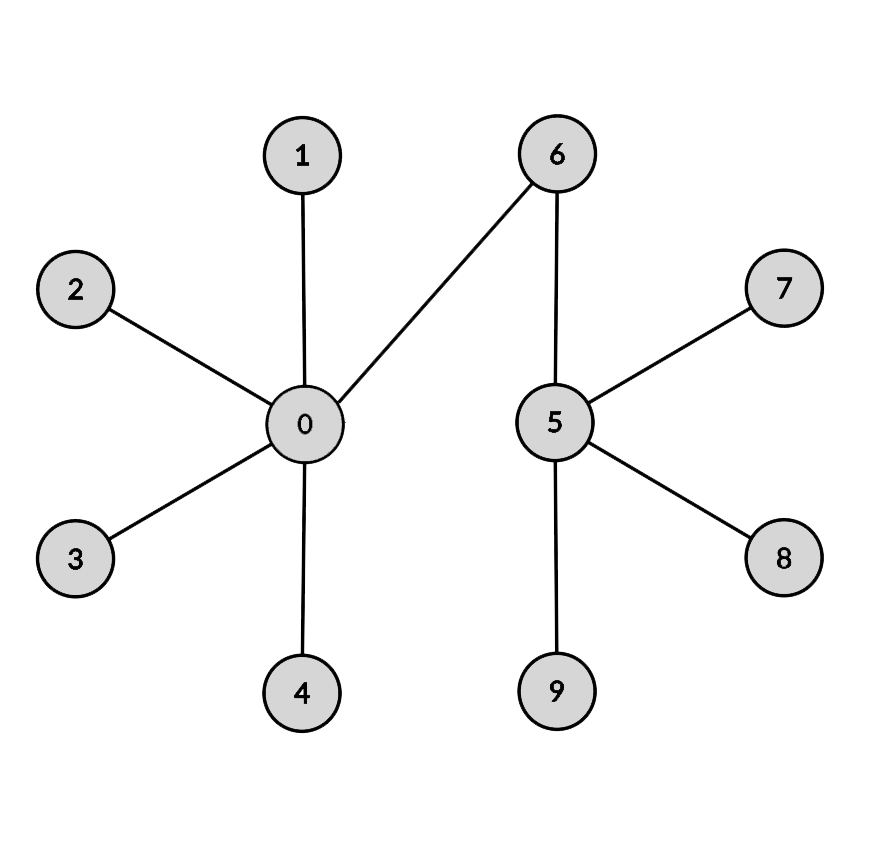
\includegraphics[height=0.15\textheight]{Figures/starC}
		\caption{}
		\label{subfig:starC}
	\end{subfigure}
	\hfill
	\begin{subfigure}[t]{0.3\textwidth}
		\centering
		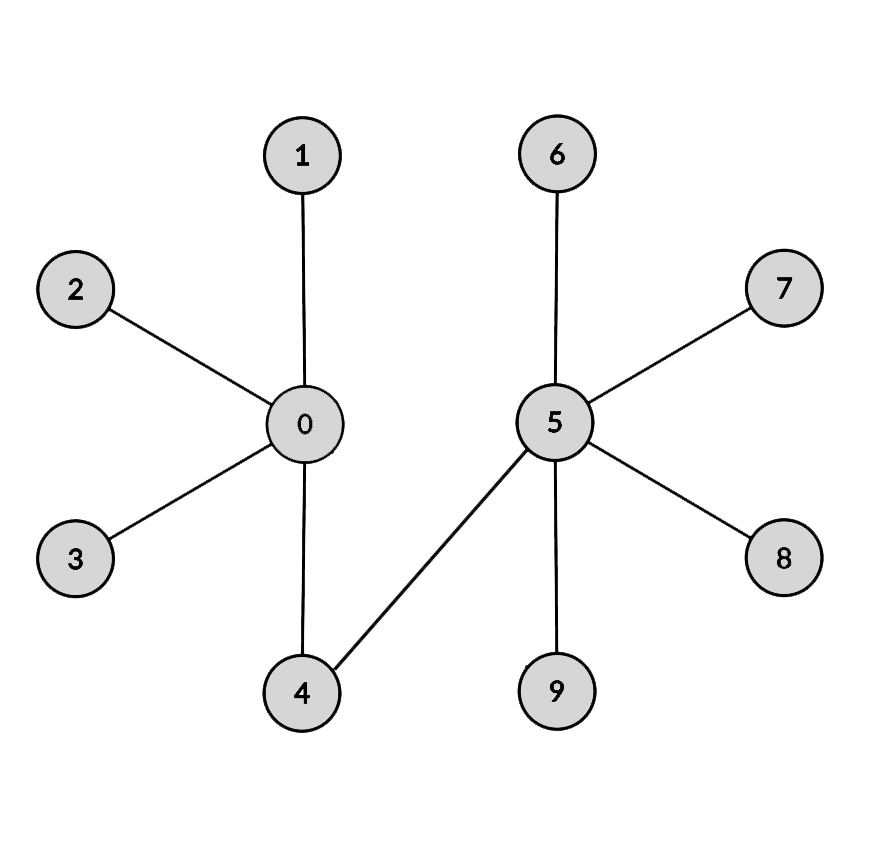
\includegraphics[height=0.15\textheight]{Figures/starD}
		\caption{}
		\label{subfig:starD}
	\end{subfigure}
	\begin{subfigure}[t]{0.3\textwidth}
		\centering
		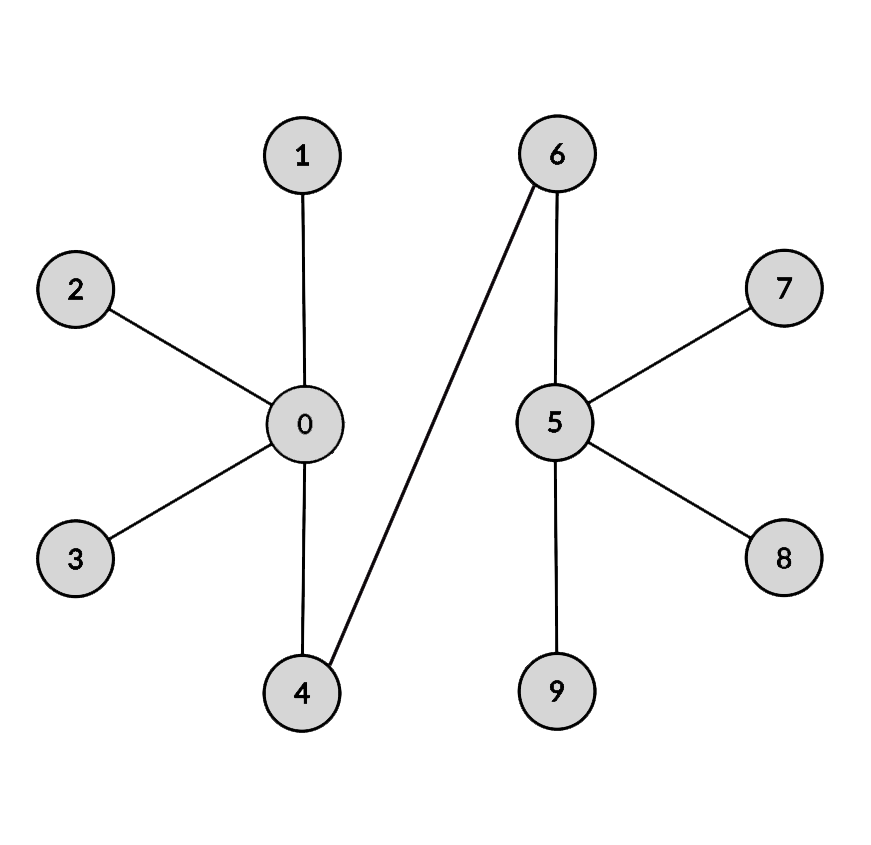
\includegraphics[height=0.15\textheight]{Figures/starE}
		\caption{}
		\label{subfig:starE}
	\end{subfigure}
	\caption{Edge addition cases}
	\label{fig:edgeCases}
\end{figure}



$case1$

\begin{equation}
	\begin{aligned}
		&Z_0 = \frac{1*(1) + 4*(1)+1*(-1)}{1 + 5} = \frac{4}{6} = \frac{2}{3}\\
		&Z_1,Z_2,Z_3,Z_4 = \frac{1*(+1) + 1*(+1)}{1 + 1} = \frac{2}{2} = 1\\
		&Z_5 = \frac{1*(-1) + 4*(-1) +1*(+1)}{1 + 5} = \frac{-4}{6} =  -\frac{2}{3}\\
		&Z_6,Z_7,Z_8,Z_9 = \frac{1*(-1) + 1*(-1)}{1 + 1} = \frac{-2}{2} = -1\\
		&||\pi(z)||^2 = 0.298142397
	\end{aligned}
\end{equation}

$case2$
\begin{equation}
	\begin{aligned}
		&Z_0 = \frac{1*(+1) + 4*(1)+1*(-1)}{1 + 5} = \frac{4}{6} = \frac{2}{3}\\
		&Z_1,Z_2,Z_3,Z_4 = \frac{1*(+1) + 1*(+1)}{1 + 1} = \frac{2}{2} = 1\\
		&Z_5 = \frac{1*(-1) + 4*(-1)}{1 + 4} = \frac{-5}{5} = -1\\
		&Z_6 = \frac{1*(-1)+1*(-1) + 1*(+1)}{1+2}=-\frac{1}{3}\\
		&Z_7,Z_8,Z_9 = \frac{1*(-1) + 1*(-1)}{1 + 1} = \frac{-2}{2} = -1\\
		&||\pi(z)||^2 = 0.29249881291
	\end{aligned}
\end{equation}


$case3$
\begin{equation}
	\begin{aligned}
		&Z_0 = \frac{1*(+1) + 4*(1)}{1 + 4} = \frac{5}{5} = 1\\
		&Z_1,Z_2,Z_3 = \frac{1*(+1) + 1*(+1)}{1 + 1} = \frac{2}{2} = 1\\
		&Z_4 = \frac{1*(+1) + 1*(-1)}{1 + 2} = -\frac{-1}{3}\\
		&Z_5 = \frac{1*(-1)+4*(-1) + 1*(+1)}{1+5}=-\frac{4}{6}=-\frac{2}{3}\\
		&Z_6,Z_7,Z_8,Z_9 = \frac{1*(-1) + 1*(-1)}{1 + 1} = \frac{-2}{2} = -1\\
		&||\pi(z)||^2  = 0.29249881291
	\end{aligned}
\end{equation}


$case4$

\begin{equation}
	\begin{aligned}
		&Z_0 = \frac{1*(+1) + 4*(1)}{1 + 4} = \frac{5}{5} = 1\\
		&Z_1,Z_2,Z_3 = \frac{1*(+1) + 1*(+1)}{1 + 1} = \frac{2}{2} = 1\\
		&Z_4 = \frac{1*(+1)+1*(+1) + 1*(-1)}{1 + 2} = \frac{1}{3} \\
		&Z_6 = \frac{1*(+1) + 1*(-1)+ 1*(-1)}{1 + 2} = -\frac{1}{3}\\
		&Z_5 = \frac{1*(-1) + 4*(-1)}{1 + 4} = -\frac{5}{5} = -1\\
		&Z_7,Z_8,Z_9 = \frac{1*(-1) + 1*(-1)}{1 + 1} = \frac{-2}{2} = -1\\
		&||\pi(z)||^2 = 0.28674417556
	\end{aligned}
\end{equation}

Therefore, the maximum decrease is achieved by the addition of node $4\rightarrow6$. Even though real graphs do not match this case exactly, they often have a structure that resembles star-graphs in certain ways: a small number of highly popular vertices receive incoming edges from a large number of other vertices \cite{garimella}.

\section{Proposed Algorithm}
\label{sec:proposedAlgorithm}

The results from section~\ref{sec:intuition} makes us consider edge addition between low-degree vertices from each side of the polarized communities. The algorithm can be seen in the figure Algorithm~\ref{alg:algorithm}.

\begin{algorithm}[t]
	\caption{Minimization of the polarization index $\pi(z)$}
	\label{alg:algorithm}
	\begin{flushleft}
        		\textbf{INPUT:} Graph $G$, number of edges to add , $k$; $k1$, $k2$, low degree vertices in each of the polarized communities in $X$,$Y$ respectively.\\
        		\textbf{OUTPUT:} List of $k$ edges that minimize the polarization index $\pi(z)$
	\end{flushleft}
	\begin{algorithmic}[1]
		\STATE $Out \leftarrow Empty List;$
		\FOR {$i = 1:k1 \ do$}
		\STATE $Vertex \ u = X[i]$
		\FOR {$j= 1:k2 \ do$}
		\STATE $Vertex \ v = Y[i]$
		\STATE Compute $\pi(z)$, the decrease if the edge $(u,v)$ is added;
		\STATE Append edge $(u,v)$ to Out;
		\ENDFOR
		\ENDFOR
		\STATE $Sorted \leftarrow sort(Out)$ by $\pi(z)$ by decreasing order;
		\STATE Return top $k$ from $Sorted$
	\end{algorithmic}
\end{algorithm}


